\documentclass[10pt]{beamer}

\usetheme{metropolis}
\usepackage{appendixnumberbeamer}

\usepackage{booktabs}
\usepackage[scale=2]{ccicons}
\usepackage{graphicx}
\usepackage{pgfplots}
\usepgfplotslibrary{dateplot}
\usepackage{caption}
\usepackage{subcaption}
\usepackage{xspace}
\usepackage{hyperref,xcolor}

\usepackage{makeidx}
\definecolor{winered}{rgb}{0.5,0,0}
\newcommand{\themename}{\textbf{\textsc{metropolis}}\xspace}

\title{Bhabha Tracking Efficiencies}
%\subtitle{A modern beamer theme}
\date{12.04.2019}
\author{Martin Sobotzik}
\institute{Johannes Gutenberg Universit\"at Mainz}
% \titlegraphic{\hfill
\includegraphics[height=1.5cm]{logo.pdf}}

\definecolor{darkblue}{rgb}{0,0,.5}
\hypersetup{pdftex=true, colorlinks=true, breaklinks=true, linkcolor=darkblue, menucolor=darkblue, pagecolor=darkblue, urlcolor=darkblue}


%citecolor={winered} %Gives errors when turned on
%allcolors={winered} %Gives errors when turned on

\begin{document}

\maketitle
{%
\setbeamertemplate{frame footer}{Bhabha Tracking Efficiencies}

%\section{Reproducing Plots}


\begin{frame}{Motivation}

\begin{itemize}	
	\item I would like to estimate the tracking efficiency 
	\item I use Bhabha events because if one track is reconstructed then the other particle should also produce a track

\end{itemize}
	\begin{equation*}
		\epsilon = \frac{\textrm{Number of Bhabha events with exactly 2 tracks}}{\textrm{Number of Bhabha events with one or more tracks}}
	\end{equation*}
	
	\begin{itemize}
		\item  This idea comes from some plots presented by Sam in previous  \href{https://confluence.desy.de/display/BI/ECL+Meetings?preview=/84320165/109161400/SCunliffe181123-ECL.pdf}{tracking and ECL} meetings.
	\end{itemize}





\end{frame}
	
\begin{frame}{Getting Started}
	
\begin{itemize} 
	\item Cuts Sam used:
	
	
	\begin{itemize}
		\item gamma:probe '$(\textrm{E} > 0.1 )$'
		\item gamma:tag '$(\textrm{clusterE} > 3.0)$'
		\item vpho:cand 'reconstructed from gamma:probe and gamma:tag'
	\end{itemize}

	
		\begin{itemize}
			\item $0.296706 < \theta < 2.61799 \rightarrow$ It has to hit the ECL
			\item $\textrm{nCleanedTracks}[ \textrm{abs}(\textrm{dz}) < 2.0 \textrm{ and } \textrm{abs}(\textrm{dr}) < 0.5 \textrm{ and nCDCHits} > 0 \textrm{ and pt } > 0.15] < 1 \rightarrow $ bad quality hits 
			\item $\textrm{M}(\textrm{vpho}) > 8.0\,\textrm{GeV} \rightarrow $ To cut away background (not from his email but surely he is using something like that)					
		\end{itemize}
	
\end{itemize}

\begin{itemize}
	\item Cuts I use:
	\begin{itemize}
		\item $\textrm{M(vpho)}>8.0\, \textrm{GeV}$ $\rightarrow$ For the vpho to have a mass of at least $8\,\textrm{GeV}$, $\textrm{gamma:tag}$ and $\textrm{gamma:probe}$ must have at least an energy of more than $3\,\textrm{GeV}$
	
	\end{itemize}
\end{itemize}

	
\end{frame}

\begin{frame}{Reproducing Plots}
	
	\begin{itemize}
		\item The plots in the following slides are produced using prod6 (this is because as a starting point I tried to reproduce Sam's plots)
		\item Sam used all Prod6 data. I am only using the following: /hsm/belle2/bdata/Data/release-02-01-00/DB00000438 /prod00000006/e0003/4S/r02*/all/mdst.sub00/*.root
		
		\item Sam's plot is on the left.	
		
\end{itemize}
	
	
	\begin{figure}
		\begin{subfigure}{.5\textwidth}
		\centering
		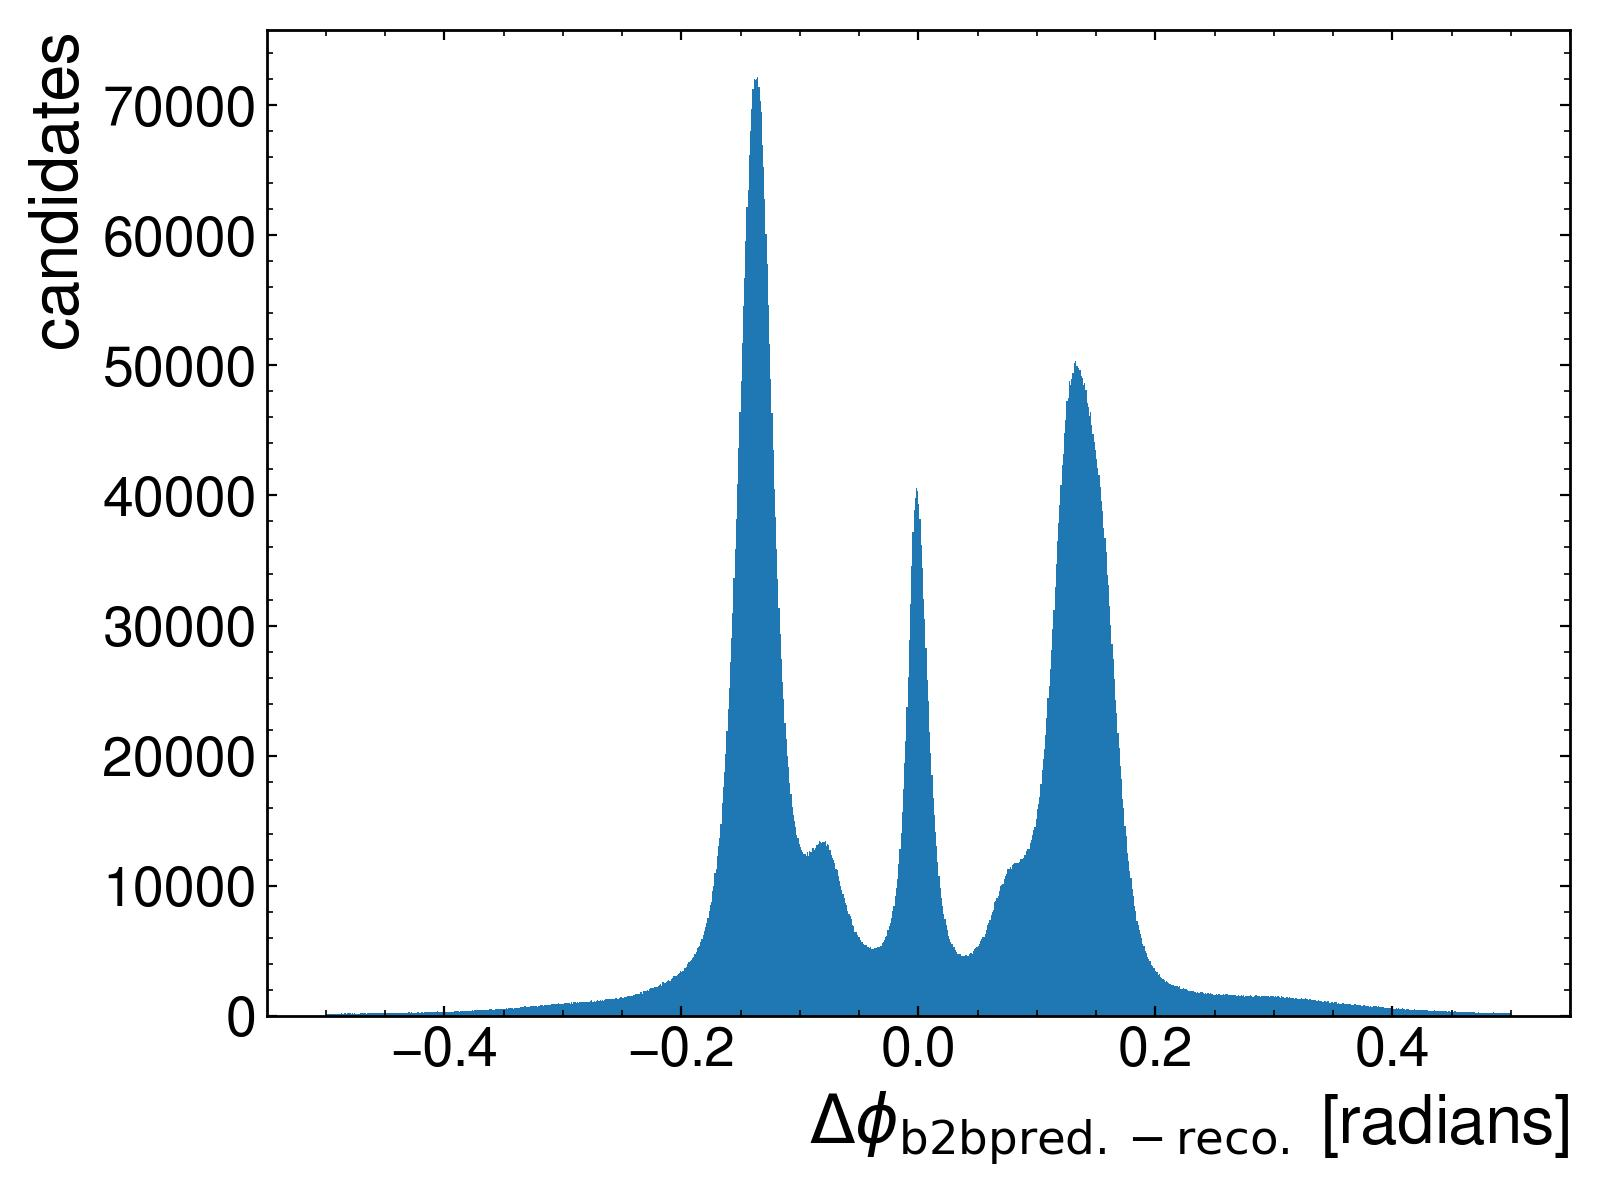
\includegraphics[width=5cm]{Plots/deltaPhiSam.jpeg}
		
		\label{fig:sub1}
	\end{subfigure}%
\begin{subfigure}{.5\textwidth}
\centering
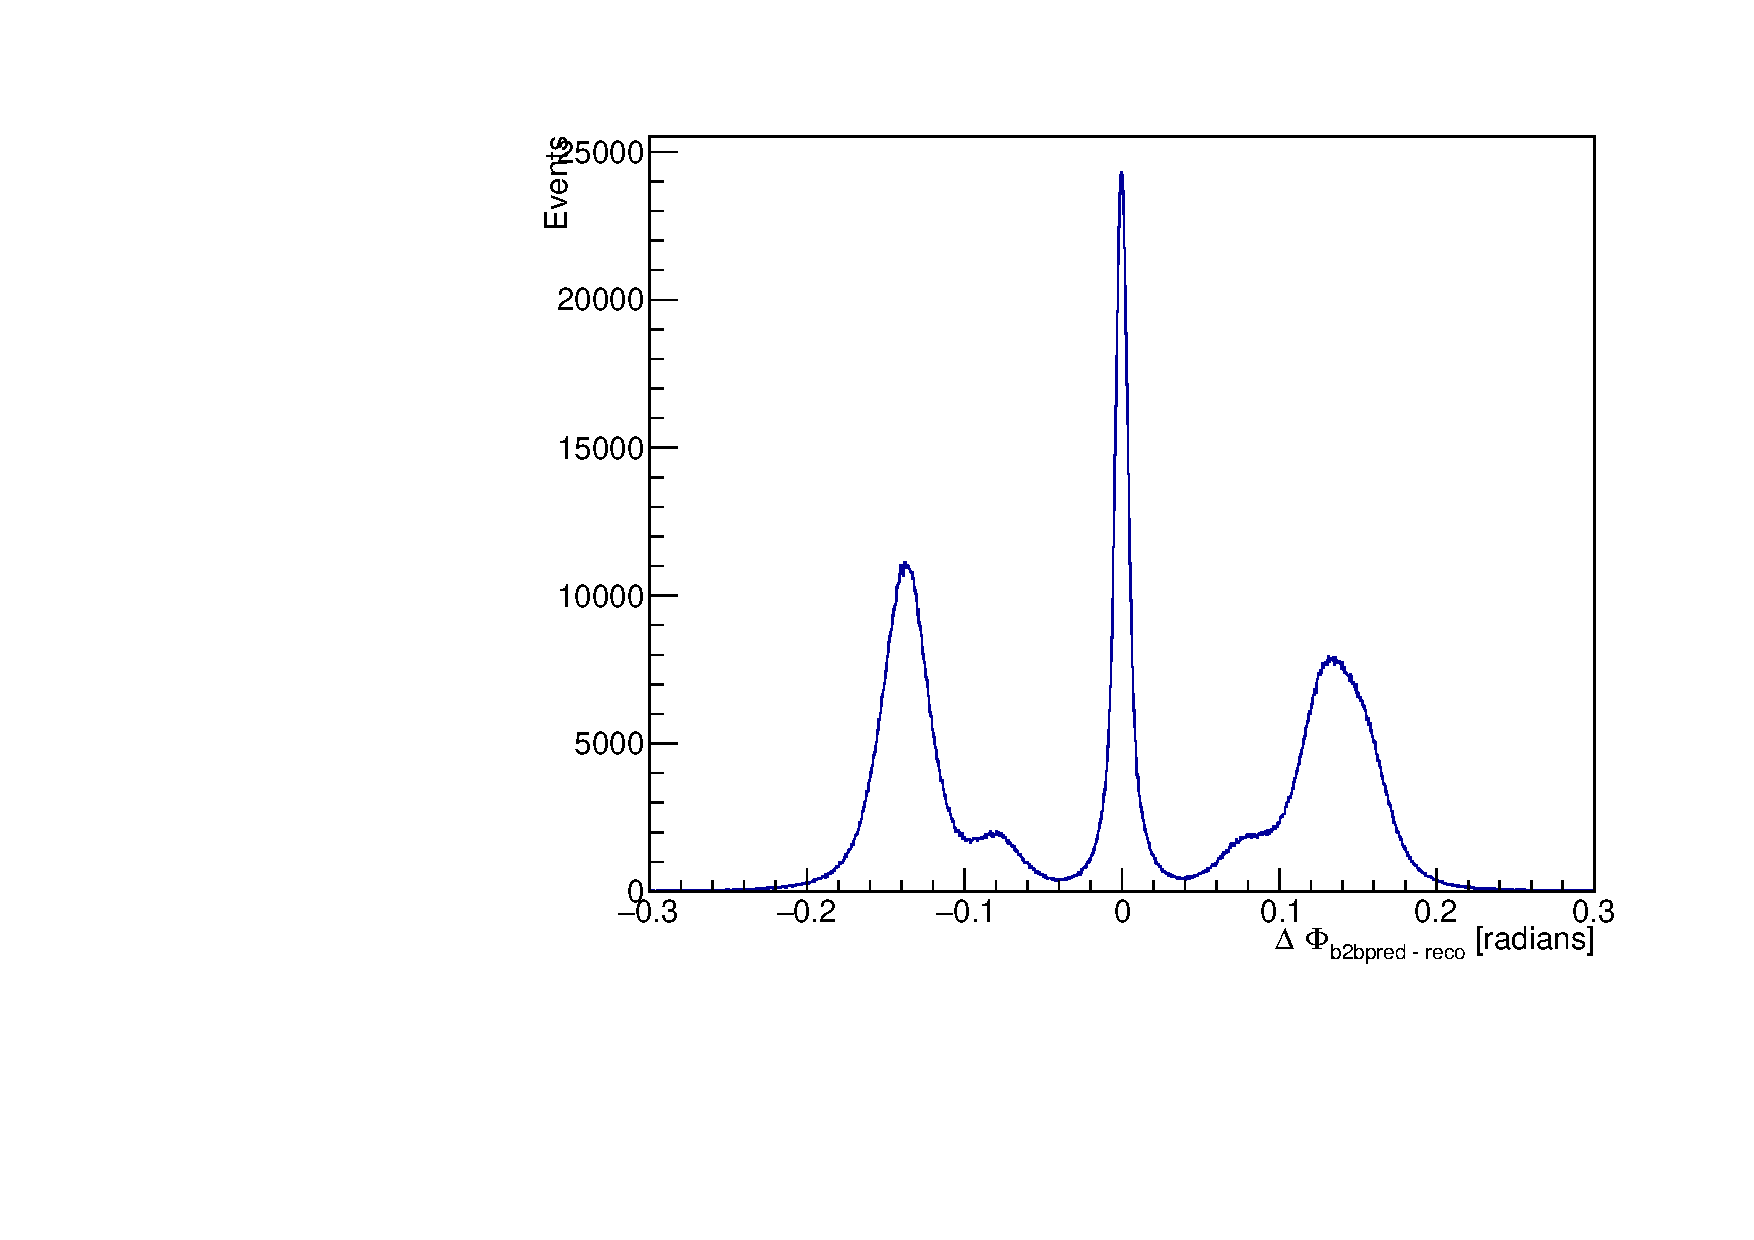
\includegraphics[width=5cm]{Plots/DeltaPhi.pdf}

\label{fig:sub2}
\end{subfigure}

\label{fig:test}
	\end{figure}
	
	
\end{frame}

\begin{frame}{Running on MC}
	\begin{itemize}
		\item At first I ran over MC11 $\textrm{ee}\rightarrow\textrm{ee}$ samples with the same steering file but I almost had no events in the gamma list
		\item 1st problem: ECL hits are written in the gamma list only if they have no track associated. Not every ECL hit is written in the gamma list
		\item 2nd problem: I also have to look at events with only one charge particle tracked $\rightarrow$ I have to \textit{reconstruct}: $\textrm{vpho}\rightarrow \gamma \textrm{e}$ and $\textrm{vpho}\rightarrow \textrm{ee}$ 
		 
	\end{itemize}
\begin{figure}
	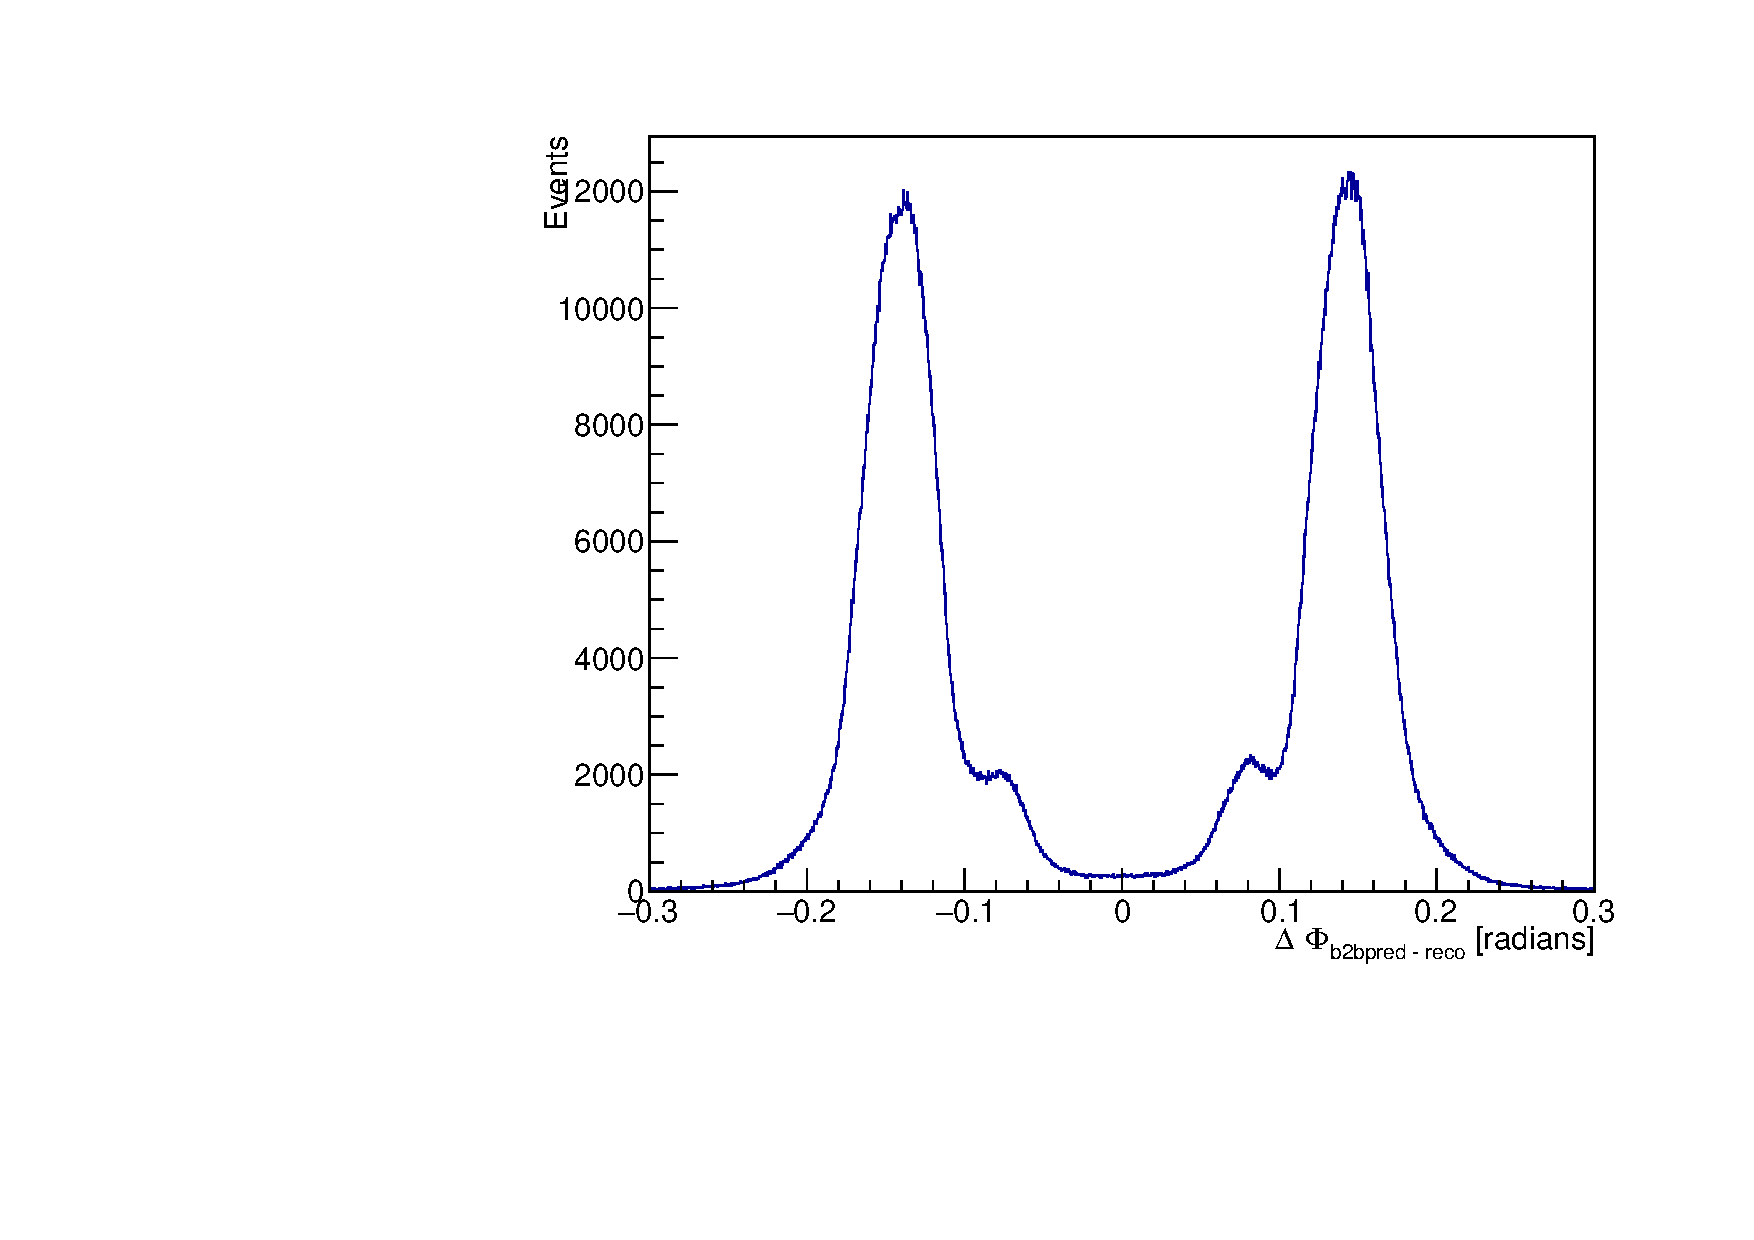
\includegraphics[width=5.5cm]{Plots/MCDeltaPhi}
\end{figure}



\end{frame}

\begin{frame}{More problems}
	\begin{itemize}
		\item<1,2> Double peak structure has to be understood 
		\item<2> Sometimes more than one vpho per event is reconstructed 
	\end{itemize}
\begin{figure}
	\includegraphics<1>[width=5.5cm]{Plots/MCDeltaPhi}
	\includegraphics<2>[width=5.5cm]{Plots/NumVpho}
\end{figure}

\end{frame}



\begin{frame}{Next steps}
	\begin{itemize}
	\item Select best vpho
	\item Cut on $\Delta \Phi_{\textrm{b2bpred -reco}}$ peak and calculate a first efficiency
\end{itemize}
\end{frame}
\end{document}
